\documentclass{sigchi}

% Use this section to set the ACM copyright statement (e.g. for
% preprints).  Consult the conference website for the camera-ready
% copyright statement.

% Copyright
\CopyrightYear{2016}
%\setcopyright{acmcopyright}
\setcopyright{acmlicensed}
%\setcopyright{rightsretained}
%\setcopyright{usgov}
%\setcopyright{usgovmixed}
%\setcopyright{cagov}
%\setcopyright{cagovmixed}
% DOI
\doi{http://dx.doi.org/10.475/123_4}
% ISBN
\isbn{123-4567-24-567/08/06}
%Conference
\conferenceinfo{UIST'18,}{May 07--12, 2016, San Jose, CA, USA}
%Price
\acmPrice{\$15.00}

% Use this command to override the default ACM copyright statement
% (e.g. for preprints).  Consult the conference website for the
% camera-ready copyright statement.

%% HOW TO OVERRIDE THE DEFAULT COPYRIGHT STRIP --
%% Please note you need to make sure the copy for your specific
%% license is used here!
% \toappear{
% Permission to make digital or hard copies of all or part of this work
% for personal or classroom use is granted without fee provided that
% copies are not made or distributed for profit or commercial advantage
% and that copies bear this notice and the full citation on the first
% page. Copyrights for components of this work owned by others than ACM
% must be honored. Abstracting with credit is permitted. To copy
% otherwise, or republish, to post on servers or to redistribute to
% lists, requires prior specific permission and/or a fee. Request
% permissions from \href{mailto:Permissions@acm.org}{Permissions@acm.org}. \\
% \emph{CHI '16},  May 07--12, 2016, San Jose, CA, USA \\
% ACM xxx-x-xxxx-xxxx-x/xx/xx\ldots \$15.00 \\
% DOI: \url{http://dx.doi.org/xx.xxxx/xxxxxxx.xxxxxxx}
% }

% Arabic page numbers for submission.  Remove this line to eliminate
% page numbers for the camera ready copy
% \pagenumbering{arabic}

% Load basic packages
\usepackage{balance}       % to better equalize the last page
\usepackage{graphics}      % for EPS, load graphicx instead 
\usepackage[T1]{fontenc}   % for umlauts and other diaeresis
\usepackage{txfonts}
\usepackage{mathptmx}
% \usepackage[pdflang={en-US},pdftex]{hyperref} なんかわからない
\usepackage{color}
\usepackage{booktabs}
\usepackage{textcomp}

% Some optional stuff you might like/need.
\usepackage{microtype}        % Improved Tracking and Kerning
% \usepackage[all]{hypcap}    % Fixes bug in hyperref caption linking
\usepackage{ccicons}          % Cite your images correctly!
% \usepackage[utf8]{inputenc} % for a UTF8 editor only

% If you want to use todo notes, marginpars etc. during creation of
% your draft document, you have to enable the "chi_draft" option for
% the document class. To do this, change the very first line to:
% "\documentclass[chi_draft]{sigchi}". You can then place todo notes
% by using the "\todo{...}"  command. Make sure to disable the draft
% option again before submitting your final document.
\usepackage{todonotes}

% Paper metadata (use plain text, for PDF inclusion and later
% re-using, if desired).  Use \emtpyauthor when submitting for review
% so you remain anonymous.
\def\plaintitle{Bridging the Translation Gap with ExpandHelp}
\def\plainauthor{First Author, Second Author, Third Author,
  Fourth Author, Fifth Author, Sixth Author}
\def\emptyauthor{}
\def\plainkeywords{Authors' choice; of terms; separated; by
  semicolons; include commas, within terms only; required.}
\def\plaingeneralterms{Documentation, Standardization}

% llt: Define a global style for URLs, rather that the default one
\makeatletter
\def\url@leostyle{%
  \@ifundefined{selectfont}{
    \def\UrlFont{\sf}
  }{
    \def\UrlFont{\small\bf\ttfamily}
  }}
\makeatother
\urlstyle{leo}

% To make various LaTeX processors do the right thing with page size.
\def\pprw{8.5in}
\def\pprh{11in}
\special{papersize=\pprw,\pprh}
\setlength{\paperwidth}{\pprw}
\setlength{\paperheight}{\pprh}
\setlength{\pdfpagewidth}{\pprw}
\setlength{\pdfpageheight}{\pprh}

% Make sure hyperref comes last of your loaded packages, to give it a
% fighting chance of not being over-written, since its job is to
% redefine many LaTeX commands.
\definecolor{linkColor}{RGB}{6,125,233}
% \hypersetup{%
%   pdftitle={\plaintitle},
% % Use \plainauthor for final version.
% %  pdfauthor={\plainauthor},
%   pdfauthor={\emptyauthor},
%   pdfkeywords={\plainkeywords},
%   pdfdisplaydoctitle=true, % For Accessibility
%   bookmarksnumbered,
%   pdfstartview={FitH},
%   colorlinks,
%   citecolor=black,
%   filecolor=black,
%   linkcolor=black,
%   urlcolor=linkColor,
%   breaklinks=true,
%   hypertexnames=false
% }

% create a shortcut to typeset table headings
% \newcommand\tabhead[1]{\small\textbf{#1}}

% End of preamble. Here it comes the document.


\def\GH{\textsf{GitHelp}}
\def\SB{\textsf{Scrapbox}}
\def\EH{\textsf{ExpandHelp}}
\long\def\tt#1{``\texttt{#1}''}

\begin{document}

\title{\plaintitle}

\numberofauthors{3}
\author{%
  \alignauthor{Toshiyuki Masui
    \affaddr{Keio University}\\
    \affaddr{Fujisawa, Japan}\\
    \email{masui@pitecan.com}}\\
  \alignauthor{Jun Kato\\
    \affaddr{AIST}\\
    \affaddr{Tsukuba, Japan}\\
    \email{junkato}}\\
}

\maketitle

\begin{abstract}
  We introduce a flexible command translation system that can generate
  a complex command string from vague keywords
  given by the user.
  %
  % Although intuitive GUI are 
  % command-line interface (CLI) is stil widely used everywhere,
  %
  When people use computers to perform tasks,
  there is usually a huge mismatch between the users' intention
  and the required action.
  % the language and vocabularies used for the task are completely different.
  When a user wants to ``make the room darker'',
  he should translate it to a real action like ``turn off the ceiling light''.
  To do so,
  he may have to ``toggle the wall switch''
  or issue a command like ``\texttt{\$ iot ceilinglight 0}''.
  If the user is a Chinese speaker, he might have to translate his intention
  ``使房黒暗'' into ``make the room darker'',
  translate it to ``turn off the ceiling light'', 
  and finally generate a command string like ``\texttt{\$ iot ceilinglight 0}''.

  People are perpetually suffering from such multi-level ``\textit{translation gaps}''.
  Translation gaps exist even for experienced computer users, but
  they are serious for vast amount of people around the world.
  %
  We propose a simple and general translation framework
  {\EH} that can be used in a wide area of situations
  where such translation is required.
  We show how our framework can be used
  in the {\GH} system
  with which user can easily generate complex \texttt{git} commands
  from fragments of users' intentions.

\end{abstract}

\category{H.5.m.}{Information Interfaces and Presentation
  (e.g. HCI)}{Miscellaneous} \category{See
  \url{http://acm.org/about/class/1998/} for the full list of ACM
  classifiers. This section is required.}{}{}

\keywords{\plainkeywords}

\section{Introduction}

Online help systems are usually hard to use because of the
vocabulary problem \cite{Furnas:1987:VPH:32206.32212}.

People don't use online help
\cite{Novick:2006:WDP:1166324.1166329}.

When we use modern artifacts,
we shoule translate our intentions into actions required for the artifacts.
When we want to watch a movie, we may pick up a DVD disk, put it into a
DVD player, push the play button, and set up the audio and the monitor.
When we feel thirsty, we may go to the kitchen, pick up a glass, and
turn the faucet on to fill the glass with water.
All the living creatures seem to be performing such translations
between intentions and actions without difficulty, but
in the modern world, people are suffering from
serious gaps between what they want to do and what they have to do.

Even when people almost know what they have to do for what they want to do,
it is often not easy to perform the task properly.
Even when people know that they can watch a movie on the Internet,
finding a movie and playing it is a difficult task for people without experiences.
% even when detailed user manuals and documents exist.
It would be nicer if they could watch a movie on the net
just by showing a vague title or attributes of the movie
in various languages.

% We can use search engines to find clues for performing the tasks, but
% it is not always easy for people in the world, since they may have
% to use different languages to look for the information.

We propose a command translation system with which users can generate a complete
command string.
%
We provide a database consisting of
pairs of
(1) the description of the task that users want to perform,
and
(2) the actual command string required by the system.
(1) can be written using regular expressions in any language,

For example, the database can include data like
\texttt{\[ heya wo kuraku suru, \% iot ceiling 0 \]}.

% やりたいことの[* 平易な表現と実行コマンドの組を用意]して[* 共有]しておいて、[* 簡単に検索/実行]できるようにする
% 表現は[* 何語で書いてあってもかまわない]
% 例えば映画作品見たいならAmazon PrimeとNetflix両方に作品があったりする
% コマンドの例でいえば何をどの順番でパイプするかいろいろ選択肢がありうる
% 全部出てくれると便利ですね(自分の知らなかったコマンド記法が学べたりする)
% いろんな候補は出ます [増井俊之.icon]
% 「Amazonでゴジラを見る」「Netflixでゴジラを見る」みたいに
% コマンドの勉強になる とは思っています [増井俊之.icon]
% そういう話は記述した方がいいかも
% `@{2 days ago}`なんて記法を知ってる人は見たことなし [増井俊之.icon]
% 今は自力で打てるようになった!
% これを[* IMEみたいなインタフェースで利用する]
% ちなIMEはアジアでは常識ね
% [* データはWikiで共有しておいて誰でも追加/修正できる]
% 自分のやり方を定義してもいい

Contributions of this paper are as follows:

\begin{enumerate}
% 各種技術を組み合わせた翻訳支援というパラダイムの提案
\item Introduction of ``\textit{translation paradigm}'' for
  generating a correct instruction to a machine from
  the user's vague intention
\item IME-like command etnry system
% やりたいことを実行するインタフェース (IME的なもの)
\item Flexible dynamic search system based on RegExp (ExpandHelp)
% そのための柔軟なインフラ (ExpandHelp)
\item Data sharing infrastructure for the translation paradigm
% 共有/編集しやすい正規表現DSLとそのインプリ(Scrapbox+)
% \item これが唯一の解決法ではないが、こういう考え方がポピュラーになって欲しい
\end{enumerate}

\section{Example: GitHelp}

We implemented the {\GH} system
with which a user can translate his vague intention in various languages
into a complete \texttt{git} command
using the {\EH} framework.

\subsection{Entering a command}

We assume that the user is using \texttt{bash} for his software
development activities.

% \begin{figure}[h]
%   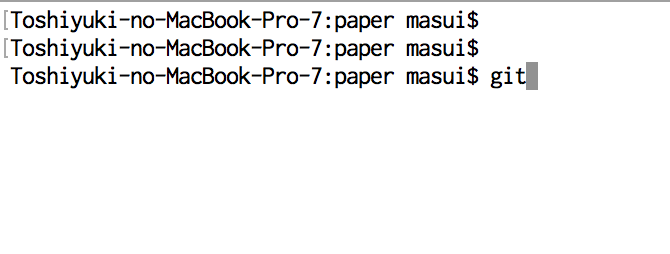
\includegraphics[width=8cm,bb=0 0 670 254]{figures/bash1.png}
%   \caption{Bash shell.}
%   \label{bash1}
% \end{figure}

When the user wants to compare the latest \texttt{README.md} file with an
older version, he tries to use \texttt{git} to show the difference.
He may know that he can use the \texttt{git diff} command to do the
conparison and invoke the following command like the following.

\begin{quotation}
\begin{verbatim}
$ git diff README.md
$
\end{verbatim}
\end{quotation}

Nothing happens, because this is not the approriate command
to compare the latest version of \texttt{README.md}
with older versions.
%
More experienced user might use a command like the following,
but it does not show anything either, because the version specification
``\verb|HEAD^^|''
specifies a file included in the older ``commit'',
and the following command only compares the \texttt{README.md}
with the with the file included in the last commit, where
\texttt{README.md} might be the same as the latest version.

\begin{quotation}
  \verb|$ git diff HEAD^^ README.md|
\end{quotation}

If {\GH} is installed,
the user can type a special key (e.g. \texttt{Cmd-Ctrl-G}) to invoke {\GH}
after typing ``\verb|git RE |'' to see how he can do the job.

\begin{figure}[h]
  % 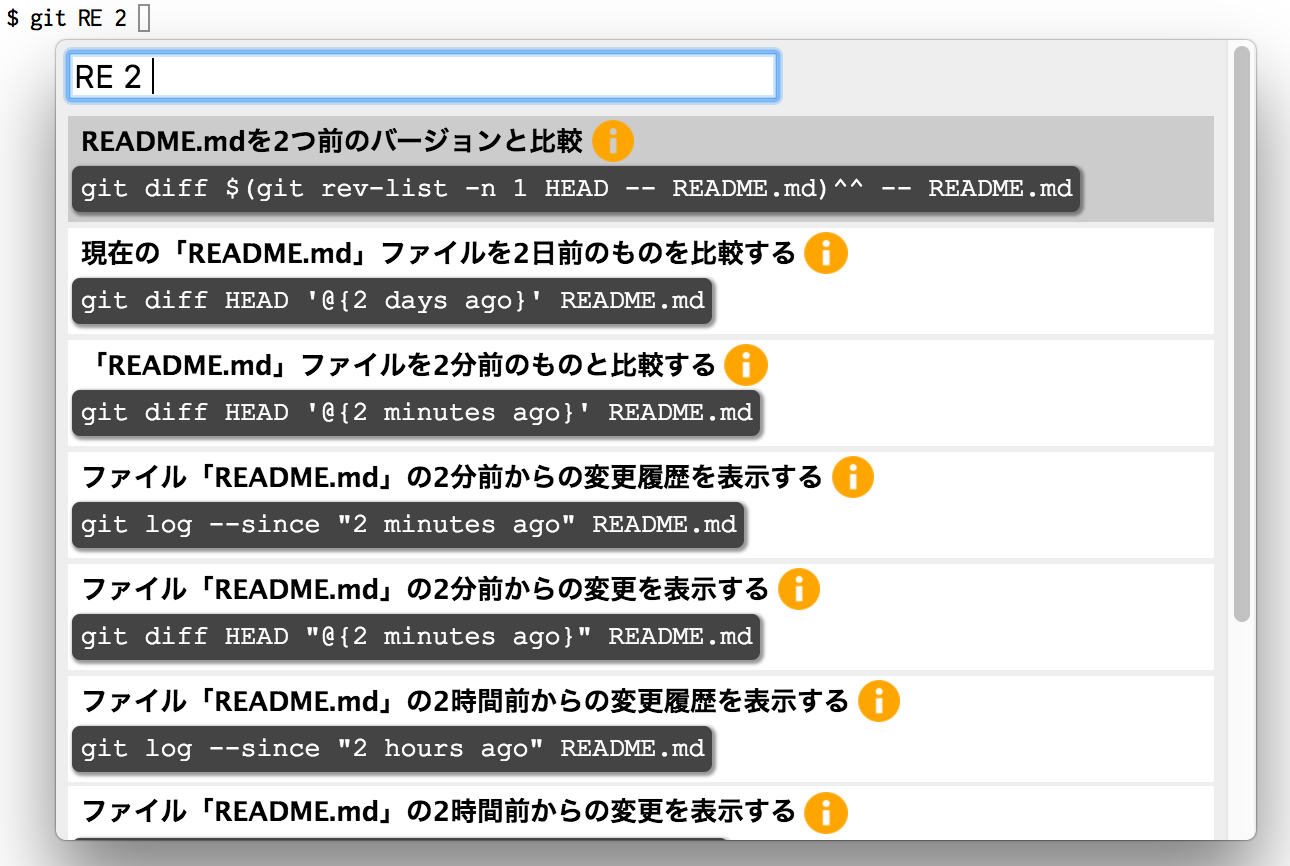
\includegraphics[width=10cm,bb=0 0 1290 866]{figures/githelp1.png}
  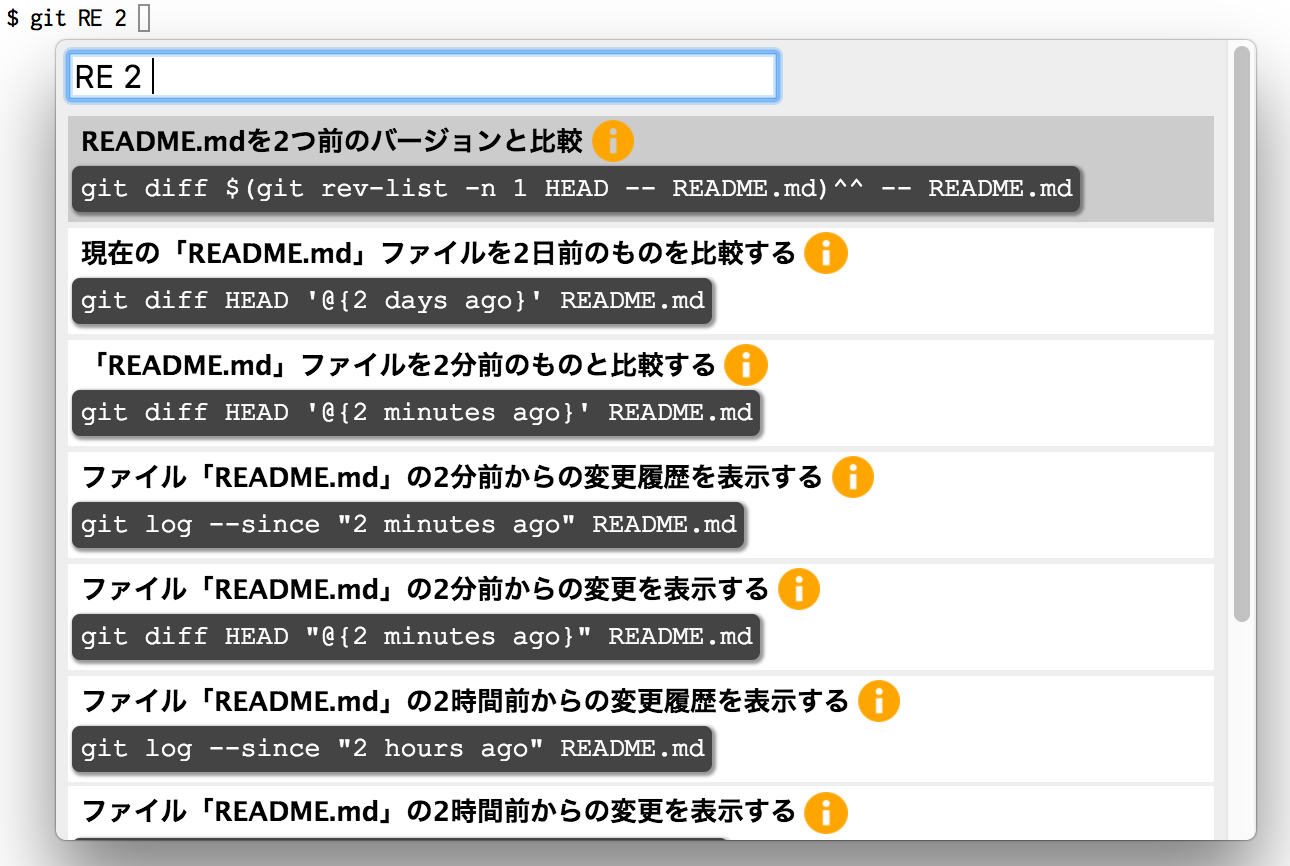
\includegraphics[width=10cm,bb=-100 -100 1190 766]{figures/githelp1.png}
  \caption{Invoking {\GH}.}
  \label{bash1}
\end{figure}

Here, various candidate entries with
descriptios and command strings are listed.
One of the entries says ``README.mdをひとつ前のバージョンと比較する'',
which means that ``to compare README with the last verson.''
%
If the user thinks that that's what he wanted to do,
he can select the entry by moving the selection by typing arrow keys
and type the enter key.
Then the command line is replaced by the correct command string
that satisfies the user's need.

A description like ``1日前''(1 day ago) was also shown in the candidate list.
This means that the user can use the same string ``\texttt{git RE 1}''
for getting the README.md file of the day before yesterday.
The command is ``\verb|$ git ... '@{1 days ago}|''.
Although such command options are very difficult to remember,
users can do the same thing only by saying \texttt{RE} and \texttt{1}.


\section{Implementation}

{\EH} implementation

\subsection{Translation}

A powerful text-search mechanism called {\EH} is used in the
background of {\GH}.

{\EH} systemm is used in {\GH}.

{\EH} is a general-purpose flexible help generation system
that has the following characteristics.

\begin{itemize}
\item Use description-execution pairs for the translation
\item Standard regular expression is used for the specification of the description
\item The specification RegExp is expanded and filtered by the user's input string
  real-time
\end{itemize}

An example of the desc-exec pair can be the following:

\begin{verbatim}
  (delete|remove) a (#{file})
  /bin/rm $2
\end{verbatim}

``remove \verb|README.md|''
into
``\verb|rm README.md|

First, the spec like \verb|#{file}| is expanded to a list of filenames like
\verb+README.md|Makefile|test.c+,
and the spec string becomes
``\verb+(delete|remove) a file (README.md|Makefile|test.c)+''.
Then this regular expression is expanded to all the possible string that match this regexp like
\begin{verbatim}
delete a file README.md
remove a file README.md
delete a file Makefile
remove a file Makefile
...
\end{verbatim}

And then all these strings are compared with the user's specification like
``\verb|del REA|'',
and if a matche is found,
this is translated to
``\verb|delete file README.md|''.

If ``\verb|destroy|'' should also be used for the spec,
the spec can be modified to 
\verb+(delete|remove) a (#{file})+.

Any kind of specs in any language can be used for the specification.
For example,

\begin{verbatim}
  #{file}を(消す|消去する)
  /bin/rm $1
\end{verbatim}

can be  used for Japanese users, who might want to delete
one of the files by specifying ``消す''.
(消す means 'delete' in Japanese).


Approximate pattern matching


\subsection{Sharing database on the Web}

The translation data of {\GH} is written on {\SB} pages on the Web.
{\SB} is a general-purpose flexible and powerful Wiki system where
users can put any kind of data for sharing.
For {\GH}, database entries like the following

(Figure)

Specs and command lines are specified with a special symbol, and
all other documents can be written just like standard manuals and help documents.

The document and the specs are written in the same document

This is
``literate programming'' style where
source codes and documents are put in the same place.

\section{Related Works}

\subsection{Input Methods}

Text input systems for non-English languages are used widely in the world, and
they are called as ``input methods'' (IMs).

\begin{figure}[h]
  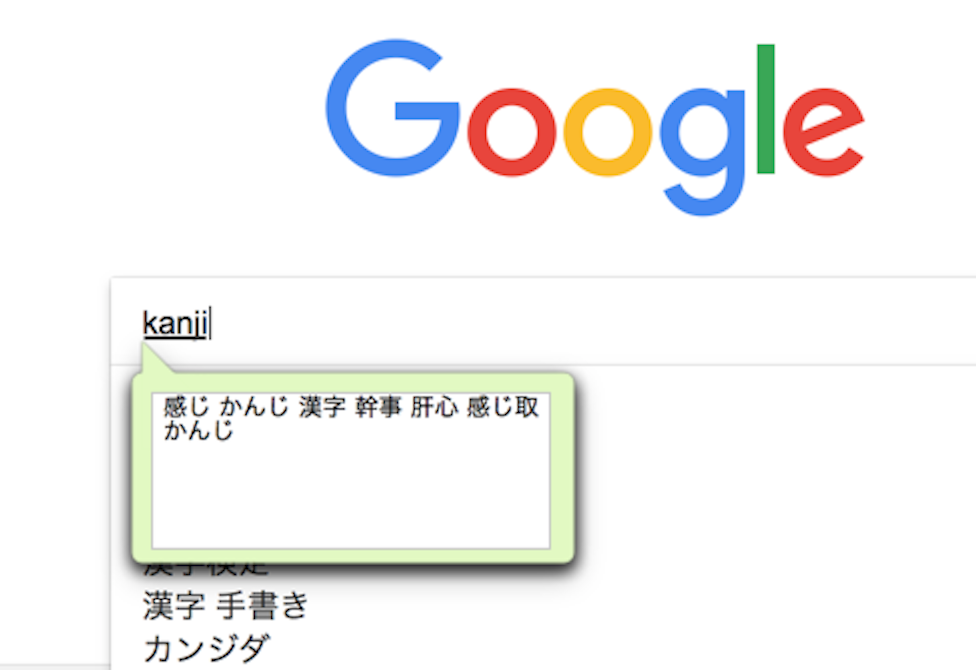
\includegraphics[width=8cm,bb=0 0 976 670]{figures/nyuuryoku-ime.png}
  \caption{An IM for Japanese text input.}
  \label{bash1}
\end{figure}

Many research and development on IMs have been performed for years, and
people are using them all the time for entering text in their mother language.

IMs are a kind of translation system that convert one
expression (pronunciation, etc.) into a textual form of a language.
In the above example, ``kanji'' will be translated to ``漢字''.

IMs are very popular especially in South-East Asian countries, and
it is very common for people there to 
use translation systems for using computers.

\subsection{Text and code completion}

On text editors an│shells,
``text completion'' has been available for a long time.
%
When a user types the TAB key after typing \tt{la} on the Unix shell,
\tt{latex}, \tt{latex}, and other commands are shown as candidates.
When a user types \tt{ls RE} and types the TAB key,
Unix shell checks the directory, find the \texttt{README.md} file, and
replace the user's input with \tt{ls README.md}.
This behavior is called ``text completion'', and many variations of
this idea have been adopted in text editors and command line editors.

User's history data can be used for 
The Reactive Keyboard system\cite{ReactiveKeyboard}
accumlates the user's command history and use the data
for predicting the user's next command.
Programing-by-Example (PBE) systems\cite{Cypher}\cite{Lieberman}.

Gitsome(https://github.com/donnemartin/gitsome)
helps \texttt{git} users by
showing possible arguments and manuals on the Unix shell,
just like {\GH}.
The goal of Git some is alomost the same as {\GH}, but
Gitsome does not support ...

\subsection{Smart IDEs}

Many smart IDEs for suggesting codes are proposed.

賢い補完
\cite{Little:2006:TKC:1166253.1166275}
% キーワードの羅列からコマンドを作成するという考えはとても正しいと思うが、実装がいかがなものか?
% キーワードぐらいは思い出せるプログラマが対象になっている
% 「margin」とか「left」とかいう単語は思い出す必要がある
% 「ちょっと字下げ」とか言っても駄目
% キーワードが違ってると駄目?
% いろいろズルをしてるようだ
% [[ActiveDocument]]はよく出てくるので特別扱いしているとか
% ステミングをしている
% ``the'' ``to'' などは捨ててるのだろう
% そもそもリカーシブな検索アルゴリズムにかなり無理がありそう
% テンプレートを作るのは大変ではないのか?

AnyCode\cite{Gvero:2015:SJE:2814270.2814295}
% [anyCode]というシステム。自然言語キーワードを入力するとコードスニペットが表示される。
% [[copy fileA fileB]]みたいなキーワードから[[FileUtil.copyFile(new File(fileA), new File(fileB))]]みたいなコード候補を生成する
% [自然言語処理]を行なっている
% [https://github.com/tihomirg/nlpcoder/tree/noola GitHub]
% 曖昧検索はできない
% 真面目に自然言語を入れる必要がある
% `123`みたいなパラメタは使えるか?
% 使えると思うが例には出てこない
% コードの説明文は出ない?
% FileUtil.copyFile(new File(fileA), new File(fileB)) と言われても、どちらが新しいファイルなのかわからない

Active Code Completion\cite{Omar:2012:ACC:2337223.2337324}
% [/ palette] と呼ばれるテンプレートを用意して[IDE]でのコード補完をサポートする
% `getDefaultColor()` を定義したいとき`purple`と入力すると、それに対応した候補が提示されるとか
% 普段使ってる環境で有益な候補が表示されると嬉しいだろうと言っている
% [[コメント]]
% [Jun Kato.icon]
% > Active code completionも思い出しました。型ごとに適した入力インタフェースを出すコード補完インタフェースのnn提案です。確か。
% [増井俊之.icon]
% IDEでどういう機能が欲しいかサーベイして設計したことになっている
% 色選択と正規表現のためのコード生成をサポートした例が紹介されている
% 一般的な補完コマンド起動によって呼び出されるようだ
% サポートウィンドウはHTML5で生成する
% しかし両者とも[/palette]の作成はかなり大変である
% 普通のユーザが作れるようなものではない
% [* 作成がすごく大変]で、[* 特定のIDEでしか使えない]という問題があると思う

Code Completion from Abbreviated\cite{Han:2009:CCA:1747491.1747530}
% [HMM]を使って正しいコードを予測して提示する
% `ch opn`みたいなテキトーな入力から`chooser.showOpenDialog()`みたいな正しいコードが候補に出る
% コードデータベースを解析
% [[コメント]]
% [増井俊之.icon] 2018/3/23 18:53
% コードのほんの一部を指定すると正しく予測されるというのは面白い
% HMMってそういうのに使えるのね
% しかし[* 関数名とか全然覚えていないときは使えないだろう]
% [語彙問題]が解決できてない
% だとすると高速入力の役にはたつが、何もかもわからない人をサポートはできない
% 用例データが存在しない場合も使えない
% [IDE]でしか使えない
% [Cyrus Omar: Active code completion]で参照されている


% 補完系IDEいろいろ
% Miller方面いろいろ

\subsection{Context-based help}

\subsection{Use cloud data for development}

BluePrint \cite{Brandt:2010:EPI:1753326.1753402}
%   サンプルコードをすぐ参照して利用できる[IDE]

Bjorn\cite{Hartmann:2010:OPS:1753326.1753478}
% 他人のヒストリを使ってコンパイルエラー対処法をサジェスト


% 他人の情報利用する系
% コード共有、コンパイルエラー共有

\subsection{Using user forums}

% Qiita, StackOverflow

\subsection{Literate Programming}

参考文献にすることはないか

Jupyter
Eve


% 文芸的プログラミング
% JavaDoc, Jupyter, Eve

\section{Evaluation}




% REFERENCES FORMAT
% References must be the same font size as other body text.
\bibliographystyle{SIGCHI-Reference-Format}
\bibliography{paper}

\end{document}
